\begin{solution}{easy}
We notice that there are certain nodes on the cube (due to symmetry), that have the same potential as illustrated below:
\newcommand{\Depth}{4}
\newcommand{\Height}{4}
\newcommand{\Width}{4}
\begin{center}
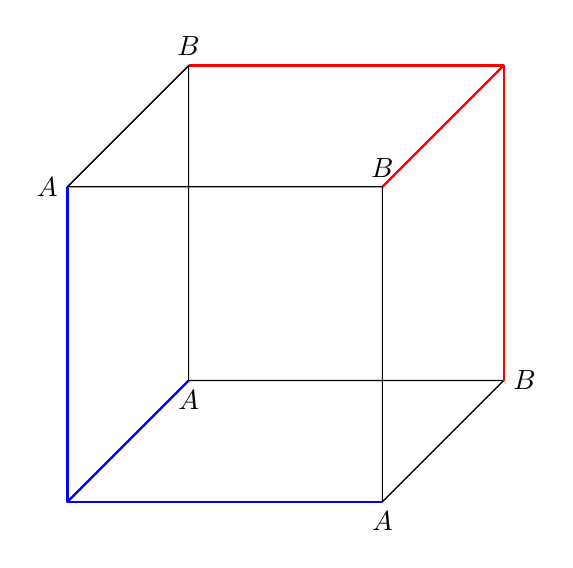
\begin{tikzpicture}
\coordinate (O) at (0,0,0);
\coordinate (A) at (0,\Width,0);
\coordinate (B) at (0,\Width,\Height);
\coordinate (C) at (0,0,\Height);
\coordinate (D) at (\Depth,0,0);
\coordinate (E) at (\Depth,\Width,0);
\coordinate (F) at (\Depth,\Width,\Height);
\coordinate (G) at (\Depth,0,\Height);

% \draw[fill=black] (C) node[left] {$C$};
\draw[fill=black] (O) node[below] {$A$};
\draw[fill=black] (G) node[below] {$A$};
\draw[fill=black] (B) node[left] {$A$};

\draw[fill=black] (F) node[above] {$B$};
\draw[fill=black] (A) node[above] {$B$};
\draw[fill=black] (D) node[right] {$B$};
% \draw[fill=black] (E) node[right] {$B$};

\draw[black] (O) -- (C) -- (G) -- (D) -- cycle;
\draw[black] (O) -- (A) -- (E) -- (D) -- cycle;
\draw[black] (O) -- (A) -- (B) -- (C) -- cycle;
\draw[black] (D) -- (E) -- (F) -- (G) -- cycle;
\draw[black] (C) -- (B) -- (F) -- (G) -- cycle;
\draw[black] (A) -- (B) -- (F) -- (E) -- cycle;

\draw[blue, thick] (C) -- (O);
\draw[blue, thick] (C) -- (G);
\draw[blue, thick] (C) -- (B);

\draw[red, thick] (E) -- (A);
\draw[red, thick] (E) -- (D);
\draw[red, thick] (E) -- (F);
\end{tikzpicture}
\end{center}
We can shortwire the connections between the ends of all resistors with the same color (e.g. identically labeled nodes have the same potential) to transform it to the following circuit:
\end{solution}